\section{Interazioni fra componenti}
	\subsection{Predizione e scrittura del risultato}
	Per rappresentare come interagiscono i componenti del nostro sistema per predire i dati e scrivere il risultato viene di seguito riportato un diagramma di sequenza che mostra l'esempio in cui l'algoritmo di predizione utilizzato è Support Vector Machine. Questo esempio risulta indicativo anche per l'algoritmo di predizione Regressione Lineare.  
	\mbox{}
	\begin{landscape}
		\begin{figure} [H]
			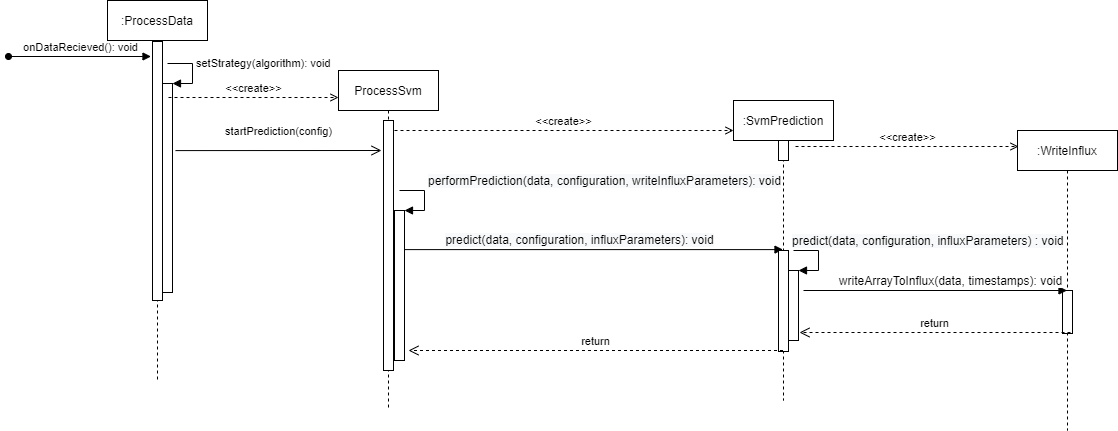
\includegraphics[width=\linewidth]{./img/Diagrammi/ds1.png}
			\caption{Diagramma di sequenza di predizione e scrittura del risultato}
		\end{figure}
	\end{landscape}
	Un'istanza di ProcessData, ricevuto il messaggio onDataRecieved(), setta il suo attributo di strategia e, di conseguenza, crea un'istanza di ProcessSvm che crea un oggetto SvmPrediction che a sua volta crea un oggetto di WriteInflux.
	L'istanza di ProcessSvm esegue quindi il metodo performPrediction(data, configuration, writeInfluxParameters) che chiama il metodo predict(data, configuration,influxParametres) sull'oggetto di tipo SvmPrediction. Quest'ultimo, ricevuti i parametri in input, esegue la predizione e chiama il metodo writeArraytoInflux(data, timestamps) su un'istanza di WriteInflux che andrà a scrivere il risultato della previsione su un database Influx.
	
	\subsection{Addestramento dell'algoritmo}
	Per rappresentare come interagiscono i componenti del nostro sistema per addestrare l'algoritmo di previsione viene di seguito riportato un diagramma di sequenza che mostra l'esempio in cui l'algoritmo utilizzato è Support Vector Machine. Questo esempio risulta indicativo anche per l'algoritmo di predizione Regressione Lineare.  
	\mbox{}
	\begin{landscape}
		\begin{figure} [H]
			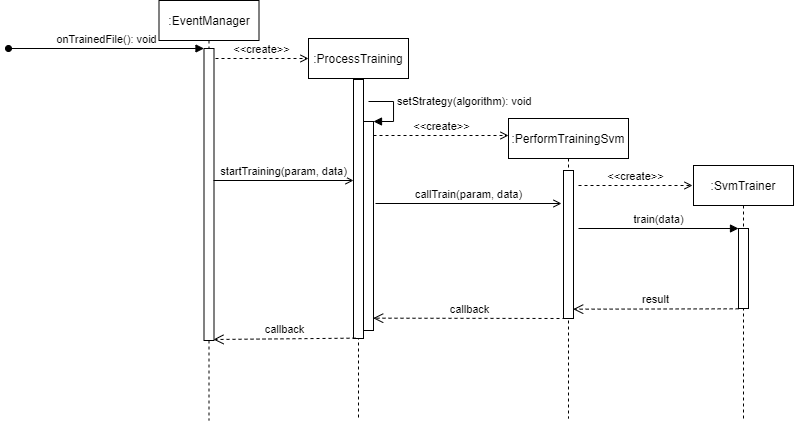
\includegraphics[width=\linewidth]{./img/Diagrammi/ds2.png}
			\caption{Diagramma di sequenza dell'addestramento dell'algoritmo}
		\end{figure}
	\end{landscape}
	Un'istanza di EventManager, ricevuto il messaggio onTrainedFile(), crea un'istanza di ProcessTraining che setta il suo attributo di strategia e, di conseguenza, crea un'istanza di PerformTrainingSvm. Quest'ultima crea quindi un oggetto SvmTrainer.
	L'istanza EventManager esegue quindi una chiamata asincrona startTraining(param, data) sull'oggetto ProcessTraining. Esso a sua volta esegue la chiamata asincrona callTrain(param, data) sull'oggetto PerformTrainingSvm che chiama il metodo train(data) sull'oggetto SvmTrainer. Infine quest'ultimo ritornerà quindi il risultato dell'addestramento.